\documentclass[handout,nooutcomes,noauthor,hints,12pt]{ximera}

\graphicspath{  
{./}
{./whoAreYou/}
{./drawingWithTheTurtle/}
{./bisectionMethod/}
{./circles/}
{./anglesAndRightTriangles/}
{./lawOfSines/}
{./lawOfCosines/}
{./plotter/}
{./staircases/}
{./pitch/}
{./qualityControl/}
{./symmetry/}
{./nGonBlock/}
}


%% page layout
\usepackage[cm,headings]{fullpage}
\raggedright
\setlength\headheight{13.6pt}


%% fonts
\usepackage{euler}

\usepackage{FiraMono}
\renewcommand\familydefault{\ttdefault} 
\usepackage[defaultmathsizes]{mathastext}
\usepackage[htt]{hyphenat}

\usepackage[T1]{fontenc}
\usepackage[scaled=1]{FiraSans}

%\usepackage{wedn}
\usepackage{pbsi} %% Answer font


\usepackage{cancel} %% strike through in pitch/pitch.tex


%% \usepackage{ulem} %% 
%% \renewcommand{\ULthickness}{2pt}% changes underline thickness

\tikzset{>=stealth}

\usepackage{adjustbox}

\setcounter{titlenumber}{-1}

%% journal style
\makeatletter
\newcommand\journalstyle{%
  \def\activitystyle{activity-chapter}
  \def\maketitle{%
    \addtocounter{titlenumber}{1}%
                {\flushleft\small\sffamily\bfseries\@pretitle\par\vspace{-1.5em}}%
                {\flushleft\LARGE\sffamily\bfseries\thetitlenumber\hspace{1em}\@title \par }%
                {\vskip .6em\noindent\textit\theabstract\setcounter{question}{0}\setcounter{sectiontitlenumber}{0}}%
                    \par\vspace{2em}
                    \phantomsection\addcontentsline{toc}{section}{\thetitlenumber\hspace{1em}\textbf{\@title}}%
                     }}
\makeatother



%% thm like environments
\let\question\relax
\let\endquestion\relax

\newtheoremstyle{QuestionStyle}{\topsep}{\topsep}%%% space between body and thm
		{}                      %%% Thm body font
		{}                              %%% Indent amount (empty = no indent)
		{\bfseries}            %%% Thm head font
		{)}                              %%% Punctuation after thm head
		{ }                           %%% Space after thm head
		{\thmnumber{#2}\thmnote{ \bfseries(#3)}}%%% Thm head spec
\theoremstyle{QuestionStyle}
\newtheorem{question}{}



\let\freeResponse\relax
\let\endfreeResponse\relax

%% \newtheoremstyle{ResponseStyle}{\topsep}{\topsep}%%% space between body and thm
%% 		{\wedn\bfseries}                      %%% Thm body font
%% 		{}                              %%% Indent amount (empty = no indent)
%% 		{\wedn\bfseries}            %%% Thm head font
%% 		{}                              %%% Punctuation after thm head
%% 		{3ex}                           %%% Space after thm head
%% 		{\underline{\underline{\thmname{#1}}}}%%% Thm head spec
%% \theoremstyle{ResponseStyle}

\usepackage[tikz]{mdframed}
\mdfdefinestyle{ResponseStyle}{leftmargin=1cm,linecolor=black,roundcorner=5pt,
, font=\bsifamily,}%font=\wedn\bfseries\upshape,}


\ifhandout
\NewEnviron{freeResponse}{}
\else
%\newtheorem{freeResponse}{Response:}
\newenvironment{freeResponse}{\begin{mdframed}[style=ResponseStyle]}{\end{mdframed}}
\fi



%% attempting to automate outcomes.

%% \newwrite\outcomefile
%%   \immediate\openout\outcomefile=\jobname.oc
%% \renewcommand{\outcome}[1]{\edef\theoutcomes{\theoutcomes #1~}%
%% \immediate\write\outcomefile{\unexpanded{\outcome}{#1}}}

%% \newcommand{\outcomelist}{\begin{itemize}\theoutcomes\end{itemize}}

%% \NewEnviron{listOutcomes}{\small\sffamily
%% After answering the following questions, students should be able to:
%% \begin{itemize}
%% \BODY
%% \end{itemize}
%% }
\usepackage[tikz]{mdframed}
\mdfdefinestyle{OutcomeStyle}{leftmargin=2cm,rightmargin=2cm,linecolor=black,roundcorner=5pt,
, font=\small\sffamily,}%font=\wedn\bfseries\upshape,}
\newenvironment{listOutcomes}{\begin{mdframed}[style=OutcomeStyle]After answering the following questions, students should be able to:\begin{itemize}}{\end{itemize}\end{mdframed}}



%% my commands

\newcommand{\snap}{{\bfseries\itshape\textsf{Snap!}}}
\newcommand{\flavor}{\link[\snap]{https://snap.berkeley.edu/}}
\newcommand{\mooculus}{\textsf{\textbf{MOOC}\textnormal{\textsf{ULUS}}}}


\usepackage{tkz-euclide}
\tikzstyle geometryDiagrams=[rounded corners=.5pt,ultra thick,color=black]
\colorlet{penColor}{black} % Color of a curve in a plot



\ifhandout\newcommand{\mynewpage}{\newpage}\else\newcommand{\mynewpage}{}\fi

\title{Hip to be square}

\author{Bart Snapp and Claire Merriman}

\begin{document}
\begin{abstract}
  We extend scaling ideas from squares and cubes to arbitrary shapes.
\end{abstract}
\maketitle

\begin{listOutcomes}
\item Understand how scaling a square changes its area.
\item Understand how scaling a cube changes its surface area.
\item Understand how scaling a cube changes its volume.
\item Understand how scaling an irregular 2D object changes its area.
\end{listOutcomes}

%% \begin{listObjectives}
%%  \item Explain the relationship between scaling lengths and scaling areas and volumes,
%% \item Learn and apply basic geometric formulas.
%% \end{listObjectives}


\begin{definition}
 The \textbf{scale factor} of a model/object is how much each linear
 dimension (meaning length, width, height) is scaled.


 The ratio of the lengths of the scaled object to the original can be written
 \[
x:1
 \]
 meaning that every length is scaled (multiplied) by a factor of $x$.
\end{definition}

\mynewpage

\begin{question}
  Let's think about scaling squares and cubes. Let's start with a
  square with dimensions $s\times s$ and cube with dimensions $s\times
  s\times s$.
  \begin{enumerate}
  \item Scale a square by a scale factor of $3$. What's the ratio of the \textbf{area} of new square to the original?
  \item Scale a cube by a scale factor of $3$. What's the ratio of the \textbf{volume} of new cube to the original?
  \item Scale a cube by a scale factor of $3$. What's the ratio of the \textbf{surface area} of new cube to the original?
  \end{enumerate}
  In each case above, \textbf{draw pictures} to help you explain why
  your answer is correct.
\end{question}
\mynewpage

\begin{question}
  Let's think about scaling squares and cubes. Let's start with a
  square with dimensions $s\times s$ and cube with dimensions $s\times
  s\times s$.
  \begin{enumerate}
  \item Scale a square by a scale factor of $x$. What's the ratio of the \textbf{area} of new square to the original?
  \item Scale a cube by a scale factor of $x$. What's the ratio of the \textbf{volume} of new cube to the original?
  \item Scale a cube by a scale factor of $x$. What's the ratio of the \textbf{surface area} of new cube to the original?
  \end{enumerate}
  In each case above, \textbf{draw pictures} to help you explain why your
  answer is correct.
\end{question}
\mynewpage

\begin{question}
  We know how squares and cubes scale, but what about weird shapes?
  Louie Llama can help us out here.  Consider this picture:
  \begin{center}
    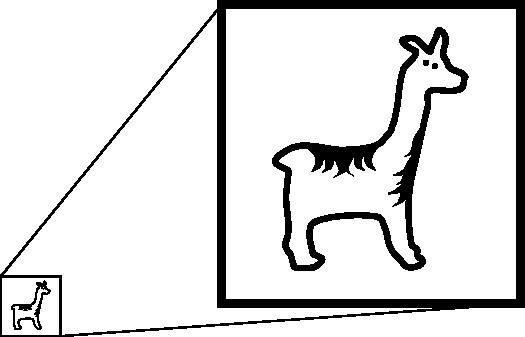
\includegraphics{llamaScaled.pdf}
  \end{center}
  Let\index{Louie Llama}
  \begin{align*}
    L &= \text{Area of Louie Llama}\\
    S &= \text{Area of Square}\\
    B &= \text{Area of bigger llama, Blouie Llama}.
  \end{align*}
  \begin{enumerate}
  \item If $x$ is the scale-factor, explain why:
    \[
    \frac{L}{S} = \frac{B}{x^2 S}
    \]
    Start by explaining what the left-hand side represents. Then
    explain what the right-hand side represents. Then explain how the
    picture helps you know that these must be equal.
  \item Solve for $B$ above, and explain how this demonstrates how
    scaling linear dimensions changes the area of \textbf{any} 2D object.
  \end{enumerate}
  
\end{question}



\end{document}
